\section{Durchführung}
\label{sec:Durchführung}
Zur Aufnahme der Franck-Hertz-Kurven auf dem Millimeterpapier werden die einzelnen 
Teile der Apparatur wie in Abbildung 3 zu sehen miteinander verbunden.
Während des gesamten Versuchs werden die Eingänge des XY-Schreibers stets so justiert, 
dass der gesamte zu untersuchende Bereich der Spannungen aufgezeichnet wird.

Zuerst wird die integrale Energieverteilung der Elektronen bei unterschiedlichen Temperaturen
untersucht. Hierzu wird die Beschleunigungsspannung $U_\text{B}$ auf $11\;\si{\volt}$ eingestellt.
Der Auffängerstrom $I_\text{A}$ wird in Abhängigkeit der Bremsspannung $U_\text{A}$
aufgezeichnet, welche von 0 bis 10 V läuft. Es wird je eine Kurve bei Zimmertemperatur und bei
eingeschalteter Heizung ($T = 140-160\;\si{\celsius}$) aufgezeichnet.

Zur Bestimmung der ersten Anregungsenergie eines Hg-Atoms werden Franck-Hertz-Kurven bei drei 
unterschiedlichen Temperaturen $T = 160-200\;\si{\celsius}$ aufgezeichnet. Hierbei
wird die Bremsspannung auf $-1\;\si{\volt}$ eingestellt und die Beschleunigungsspannung
läuft von 0 bis 56\;\si{\volt}. Es wird der Auffängerstrom in Abhängigkeit der Beschleunigungsspannung
aufgezeichnet.

Zur Ermittlung der Ionisationsenergie von Hg wird die Bremsspannung auf $-30\;\si{\celsius}$ eingestellt,
wodurch die erzeugten Ionen von der Auffängerelektrode regstriert werden, die Elektronen jedoch nicht.
Die Messung findet bei $T = 140-160\;\si{\celsius}$ statt und es wird erneut der Auffängerstrom in 
Abhängigkeit von der Beschleunigungsspannung aufgezeichnet.

\begin{figure}[H]
  \centering
  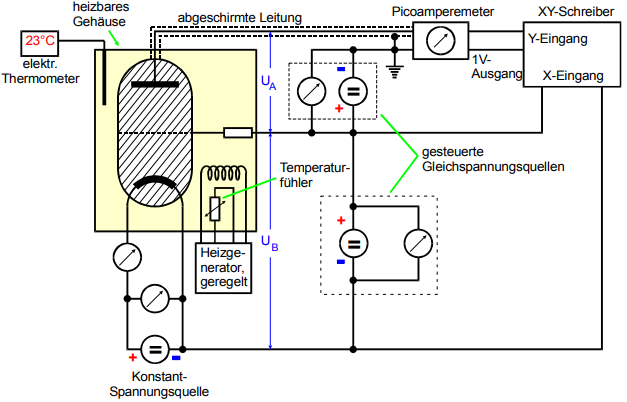
\includegraphics[width=13cm]{durchf.png}
  \caption{Versuchsaufbau zur Aufzeichnung einer Franck-Hertz-Kurve. \cite[S.124]{kent}}
  \label{fig:durchf}
\end{figure}